%!TEX root = ../main.tex

% Abstract: we conclude the benefits in each period and give future challenges

% 


\begin{figure*}[!t]
\centering
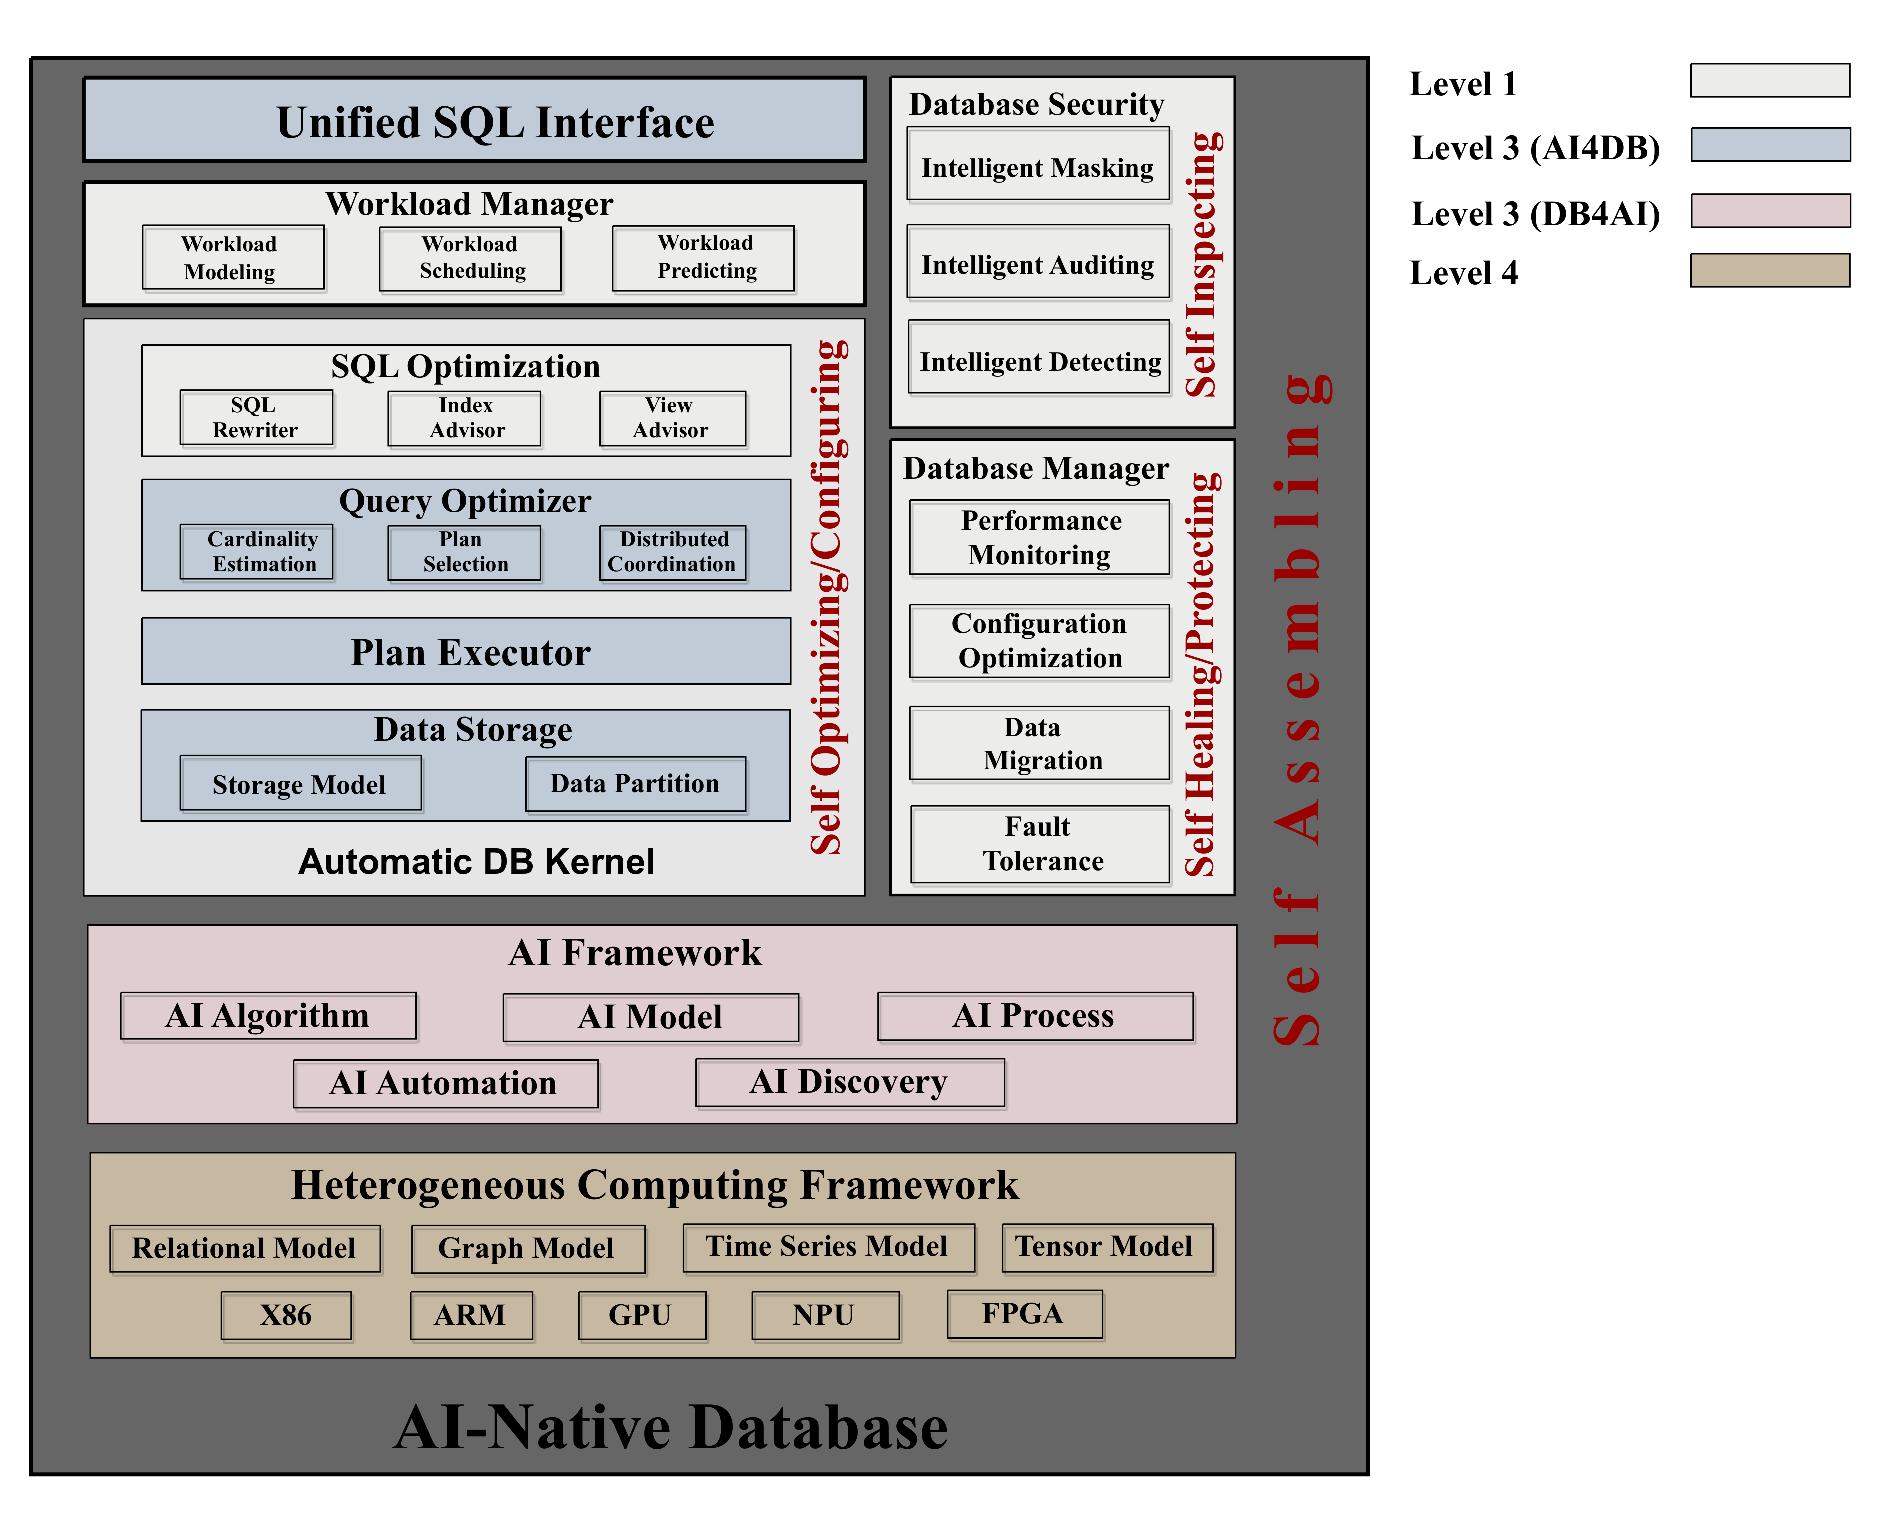
\includegraphics[width=1.0\textwidth, height=0.92\textwidth]{figs/ANDB-arch.eps}
\vspace{-1em}
\caption{The architecture of AI-Native databases}
\label{fig:ANDB}
\vspace{-1em}
\end{figure*}

 
To alleviate the issues talked above, in this section we propose a design of AI-native database, which better provides DB and AI services in five levels. 


\subsection{Level 1: AI-Advised Database}
\label{subsec: advised}
As shown in Table~\ref{tbl:ANDB}, in the first level, our database is AI-Advised, which provides auxiliary optimization of the database through suggestions~\cite{DBLP:conf/sigmod/AkenPGZ17, DBLP:journals/corr/abs-1802-00884, DBLP:conf/vldb/qtune19}.
It has an AI engine packing AI tools, which are loosely coupled with database in the form of plug-in. Limited by available resources, the AI engine mainly provides auxiliary tools from four aspects. 

$\circ$ \textbf{Workload Management}. It has two functions: to schedule user workloads and summary workload characters for the other modules. 
For \texttt{workload modeling}, traditional cost models are mostly based on empirical formulas, which have poor adaptability to different physical environments. Therefore, the machine learning model can be used to analyze and evaluate the current workload situation and future overhead, and dynamically adapt to the external environment based on gradient changes.
For \texttt{workload scheduling}, in traditional databases, resource scheduling depends heavily on parameters related to resource control, such as workspace size, maximum concurrent IO number, and etc. But these parameters are static and need to be manually configured. So we can use reinforcement learning to learn relations between database state (physical/logical), workload and database resources, and provide a reasonable and robust scheduling mechanism.
For \texttt{workload predicting}, workload usually dose not change in a fixed pattern. Traditional workload predicting methods are usually grasped by database experts according to statistical data, which can not guarantee high accuracy. So we proposed to use machine learning method for workload forecasting~\cite{DBLP:conf/sigmod/MaAHMPG18}, which can have better adaptability to different workloads. 
%In order to avoid using CPU, IO and other system resources as workload metrics in different hardware environments, we use logical metrics to characterize workload, which further ensures the stability of prediction.

$\circ$ \textbf{SQL Optimization}. It is to optimize database in SQL level. 
For \texttt{SQL rewriter}, SQL rewriter helps optimizer to choose efficient query plans by changing the way SQL is written. This level is often completed manually, which is impractical for heavy workload. So we provide a rewriting tool to learn the principles of SQL writing (e.g., avoiding full table scanning, selecting indexed columns as joins, and using table variables) and optimize the SQL structure. 
For \texttt{index advisor}, index is very important to improve the efficiency of retrieval tasks on complex data sets~\cite{DBLP:journals/kais/GaniSSH16}. However, the commonly used indexes are universal data structures. They do not analyze and utilize the distribution of data. So through machine learning, we can learn a model that reflects data patterns, and can automatically synthesize a special index structure at a lower cost.
For \texttt{view advisor}, given a set of queries, extracting high-frequency sub-queries and establishing materialized views to improve the performance of the database is very helpful. 
The traditional method caches at the whole query level, and the hit rate is low.
We construct the ML algorithm of sub-query selection according to the actual constraints so as to improve the query efficiency of batch SQL tasks.

$\circ$ \textbf{DB Manager}. It provides services (e.g., performance monitoring, tuning, fault tolerance) to ensure the stable operation of the database. In distributed scenario, high load pressure will lead to a sharp increase in failure rate, which brings great challenges to database maintenance. 
For \texttt{performance monitoring}, it automatically monitors the status of the database system (e.g., the number of batch requests per second, the number of user connections, network transceiver efficiency). Then it analyzes those indicators using machine learning algorithms. 
%Generally speaking, it includes four kinds of methods: real-time monitoring, timing monitoring, analysis report, tracking and data collection. Performance monitoring is not only statistical indicators, but also needs to understand the operation of the system based on these indicators. 
For \texttt{tuning}, database configuration involves hundreds of tunable system parameters, which control the database components in many aspects. Traditional tuning methods~\cite{DBLP:journals/pvldb/DuanTB09, DBLP:conf/cloud/ZhuLGBMLSY17} either relies on human beings (DBA-based), or cannot utilize history information (search-based). So we use a deep-reinforcement-learning-based tool~\cite{DBLP:conf/vldb/qtune19} to learn relations between database state, query and parameters, which can adapt to environment changes dynamically.
For \texttt{fault tolerance}, it includes a variety of strategies for resolving failures of hardware, transactions and system. In case of data error, the system needs to cancel the corresponding transactions in time. So we use a ML-based tool to monitor the changes caused by typical failures and realize pre-alerts. 

$\circ$ \textbf{DB Security}. It is to combine information security, cryptography technology with AI tech to  ensure the security of database. 
For \texttt{intelligent masking}, it is to hide privacy data such as ID number.  Intelligent masking technology only uses the high-dimensional, non-linear data inside the neural network to help improve the effect of data hiding. For example, in the research project conducted by Stanford University and Google, satellite images have been converted into high-frequency signals that are not easily detected. 
For \texttt{intelligent auditing}, it optimizes the auditing work from two aspects: data preprocessing and dynamic analysis. Traditional audit work often requires auditors to obtain a large number of business data. This part of the data understanding work is a waste of human resources. Intelligent auditing not only saves manpower cost, but also helps auditors to make better decisions by providing useful information from massive data.  
For \texttt{intelligent detecting}, it can automatically detect system vulnerabilities. Known intelligent detecting technology is mainly to retrieve through security scanning, while unknown security vulnerabilities need to do a lot of retrieval and testing work.  Using machine learning algorithm to discover security vulnerabilities~\cite{DBLP:journals/corr/abs-1902-10680}, it can not only detect most known vulnerabilities in national vulnerability database, but also predict and evaluate potential vulnerabilities.

\subsection{Level 2: AI-Assisted Database}
\label{subsec: assisted}
In the second level, our database is AI-Assisted, which is embedded into the database kernel for runtime optimization. AI components (e.g., tuning model, workload scheduling, view advisor)  can be merged into the corresponding database components~\cite{DBLP:journals/corr/abs-1903-01363}. This way, AI processes are integrated into the working procedure of the database. For example, if embedding the tuning model into the query optimizer, every time we generate the query plan, we can first conduct query tuning (adjust user-level parameters to better adapt to the incoming query characters), and then normally generate and execute query plan. The advantage of AI-Assisted database is that 1) it can provide more fine-grained optimization; 2) by embedding AI engine into the kernel, it can reduce much overhead such as communication cost.

However, neither Level 1 or 2 is a real AI-native database. Because the main components and organizing mode in those databases are still based on traditional methods. There are huge gap between AI technologies and databases. Starting from the third level, we introduce how to integrate intelligence integration, heterogeneity into database design to achieve the AI-native database.

\subsection{Level 3: AI-Enhanced Database}
\label{subsec: enhanced}
In the third level, our database is AI-Enhanced, which embeds intelligence and integration into database design. 
Firstly, we propose an intelligent database kernel, which implants AI into the design of database kernel. Secondly, we propose a  unified engine for both AI and DB, with which clients can use AI as easily as they use a DB.

\subsubsection{Intelligent Database Kernel}
\label{subsubsec: intelligent}
We present the design of an intelligent database kernel that enables self-configuring, self-healing, self-optimizing, self-protecting, self-inspecting and finally achieves self-organizing.

$\circ$ \textbf{Self-configuring}. Database can automatically adjust their own configuration to adapt to environment changes, including tuning parameters, upgrading software,adjusting partitioning/replication scheme, reorganizing tablespace and etc. Each function is embedded into particular DB modules to work as part of the processing.  For example, to realize tuning in query level, we embed tuner into optimizer. Each time a parse tree is input into our optimizer, it first configures parameters based on the query features and then actually generates the query plan. This way, it not only helps to generate better query plan, but prepares suitable environment for executing the query plan. 

$\circ$ \textbf{Self-healing}. Database can automatically detect, diagnose, alert and recover from DB problems (e.g., poor performance, hardware/software failovers). It adopts advantages of tools in AI-Advised DB to fully save humans from the failure-recovery loop. Firstly, it takes protective actions ahead of time (e.g., backup, data sharding, reosurce scheduling). Secondly, it can recover services even if emergency occurs (e.g., live migration).


%For example, rather than cleaning dirty pages in memory every fixed time, we replace the timing part  with the results of workload forcasting, which can predict how the workload varies. And it conducts cleaning when DB is free.live migration, checkpoint,  logging each write operations, we can focus on recording 

$\circ$ \textbf{Self-optimizing}. Database can automatically collect statistics of queries and optimize database performance in multiple granularities. Firstly, it collect statistics used in optimizer to learn current workload, which can benefit from cardinality estimation and workload scheduling. Secondly, it automatically design index, materialized query table (MQT) and data partition, which can directly optimize performance of single query. Thirdly, it automatically controls the flow of queries with query patroller to achieve overall optimization.

$\circ$ \textbf{Self-protecting}. Database can automatically monitor processing procedure of each query and prevent potential damage in time. For example, it can throttle service requests which compete resources to cut down deadlock and average waiting time; and it can kill / lower the priority of run-away queries (execution time is far longer than that estimated by the optimizer) to prevent from using up system resources.

$\circ$ \textbf{Self-inspecting}. Database can automatically monitor database state and conclude operating rules by itself. It can check database state (e.g., data consistency, DB health) all the time. And by concluding all the failover conditions and solutions, it can translate the experience in the form of publication of instrumentation data in favor of human understanding.


$\circ$ \textbf{Self-organizing}. For current databases, each level of service (e.g., parser, optimizer and executor) has multiple standardized components to choose from. How to choose the appropriate processing path for one or a batch of queries becomes meaningful. 

So we propose a self-organizing module. For different queries, we can dynamically select the appropriate components in each layer of service and assemble the appropriate execution path.
The execution path can be seen as a natural language sequence (NLS), such as $\langle$ $SQL_i$, parser$\_$pg, optimizer$\_$RBO, storage row, accelerator $\rangle$, in which each position has only discrete token options. So the problem is how to generate NLS in query level. One method is to use RL algorithm. It takes the whole path sequence as an episode and a single action as an epoch. Under each epoch, the agent chooses the next component (action), which executes the query, leading to a state transition (e.g., the query status changes into syntax tree). In this problem, action is discrete, so DDQN algorithm~\cite{DBLP:conf/aaai/HasseltGS16} can be used. Compared with other RL algorithms with discrete output, DDQN eliminates the problem of overestimation (deviate greatly from the optimal solution) by choosing decoupling actions and calculating the target Q value.

However, RL-based routing algorithm has two problems. 
Firstly, Q network will not score until the last node is generated. It is insensitive to the choice of intermediate nodes. However, for the entire path, it is necessary to give action a comprehensive score on current and future impacts. 
Secondly, when training with epoch as a unit, each node of a path is scattered in a training sample, instead of being used as a whole to calculate the gradient. 

Generating antagonistic network (GAN)~\cite{DBLP:journals/corr/abs-1902-05687} can better solve those problems of end-to-end path selection. We use G network to generate path vectors based on workload, database state and component characteristics, and we use D network as the performance model. 
But the traditional GAN network model is not fully applicable to our problem. Because it is mainly used to generate data with continuous range of values, and it is difficult to generate path vectors with discrete tokens. That is because G-networks need to be fine-tuned based on gradient descent and regress towards the expectation. But when the data is discrete tokens, fine-tuning is often meaningless.
So we choose to combine RL algorithm with GAN~\cite{DBLP:conf/aaai/YuZWY17}. Firstly, G network is used as agent in RL algorithm: action is the next service node; state includes not only query status, database status, but also generated node information. Each iteration generates a complete path. Secondly, unlike pure RL algorithm, each action is scored by D network to guide the generation of the whole path sequence.

\subsubsection{Unified Engine for AI and DB}
\label{subsubsec: engine}
After achieving the intelligent database kernel, we gain real integration by providing unified engine for DB and AI. AI and DB are closely connected. For DB, as talked above, AI can make DB  smarter. For AI, DB stores large scale of data for training the ML models. 
So it becomes easy when we can call ML model with SQL statements. Firstly, SQL is easy to use, with which technicians with basic SQL knowledge can complete most of traininig and predicting tasks. Secondly, it saves people from frequently switching between different languages of systems, when we need to write SQL to fetch data and run python scripts to run ML algorithms.

For this work, there have been some products such as BigQuery ML~\cite{DBLP:conf/ideas/FernandesB15}, SQL for DL and SQLFlow. Considering the Pros and Cons of these works, we propose an extended DB engine to achieve the following aims:

$\circ$ \textbf{AI Support}. Firstly, SQL Parser should extend SQL syntax to utilize AI methods, including model creating, training and predicting. Besides, it should minimize the use of other scripting languages (e.g., Python and R). Secondly, we extend the relational algebra theory to support both relational and tensor data models. This way, DB can support tensor processing, which is largely used in the training of AI models.


$\circ$ \textbf{General Purpose}. SQL parser should contain an abstract layer which maintains a loose couple with lower components. This way, it can be easily used on different SQL engines (e.g., PostgreSQL, Flink and Hive) or machine learning toolkits (e.g., TensorFlow, Keras and scikit-learn). 

$\circ$ \textbf{Custom Style}. Besides general operators such as SELECT and WITH, we also allow user to define how to train, evaluate and predict the ML models with user-defined functions. And they also can cache the trained model with materialized views.

The general workflow is as follows. Firstly, SQL Parser parses a SQL statement and produces a general-purpose query plan. Based on the operators in the plan, it decides whether it is for manipulating data or calling ML models. If for manipulating data, the query plan is sent to the DB executor and be executed. Otherwise, it is sent to the AI executor and be executed.

This way, database can also provide AI services in an end-to-end way. As table~\ref{tbl:AI} shows, Database supports AI services in five levels.
%Presently, DB mainly serves for structured data analysis such as financial transactions. By embedding AI algorithms into DB engine, DB can directly support many AI applications (e.g., image comparison, graph computing) in an end-to-end way. As Figure~\ref{fig:DB4AI} shows,  

$\bullet$ \textbf{DB-based AI Algorithm}. Database provides ML tool-kits and libraries (e.g., TensorFlow, Scikit-learn). Clients can write AI algorithms in UDFs or stored procedures. And they can call them repeatedly from database. 

$\bullet$ \textbf{DB-based AI Model}. Database provides classic AI models (e.g., random forest, RNN, DDQN). Clients can directly call AI models from database and only focus on the training part. 

$\bullet$ \textbf{DB-based AI Process}. Database further provides AI processes, which not only include the mature AI models but the training methods (e.g., SGD, Adam, reinforcement learning). Clients can directly call AI processes from database, only with data as input. Database automatically fine-tunes AI model using corresponding training method, and utilizes the model to produce results. 

$\bullet$ \textbf{DB-based Automation}. Database can automatically parse the requirements in AI and call proper process to solve it. Clients only need to declare their requirement. For example, if we hope to search some images, we just declare the conditions and data sources with SQL. And database automatically chooses the CNN model to conduct the work, which is also a part of the query plan.

$\bullet$ \textbf{DB-based Discovery}. Database offers an insight into the data schema and application queries, and optimizes itself with AI techniques. For example, if a new workload comes, database can call a DRL-based tuner to adjust the system parameters based on the query features, including cost estimation, resource allocation, concurrency  control and etc. 

\begin{table}[h]
\vspace{-1em}
\centering
\caption{Five levels of machine learning consumability in DBMS}
\label{tbl:AI}
{%\footnotesize
  \hspace*{-0em} \begin{tabular}{|c|c|l|c|c|}\hline
  
\multirow{2}{*}{\textbf{Level}} & \multirow{2}{*}{\textbf{Consumability}} & \multirow{2}{*}{\textbf{\ \ \ \ \ \ \ \ \ \ \ \ \ \ \ \ \ \ \ \ \ \ \ \ Description}} & \multirow{2}{*}{\textbf{Target Users}} & $\textbf{ML Skill}$ \\
 &  &  & & $\textbf{Level}$ \\\hline

\multirow{2}{*}{\textbf{1}} & \multirow{2}{*}{Algorithm} & \multirow{2}{*}{Algorithms as UDFs and stored procedures} & Data scientists,  & \multirow{2}{*}{High} \\
 &  & & experienced developers & \\\hline


\multirow{2}{*}{\textbf{2}} & \multirow{2}{*}{Model} & Models as first-class object with DDL, & App. developers  & \multirow{2}{*}{Medium} \\
 &  &  DCL, DML capability  & and DBAs & \\\hline

\multirow{2}{*}{\textbf{3}} & \multirow{2}{*}{Process} &  Processes as first-class object with DDL, & App. developers & \multirow{2}{*}{Low} \\
 &  & with DCL, DML capability  & and DBAs & \\\hline

\multirow{2}{*}{\textbf{4}} & \multirow{2}{*}{Automation} &  Problem specifications as first-calss object & Business specialists, DBAs & \multirow{2}{*}{Low} \\
 &  & with DDL, DCL, DML capability  & app. developers & \\\hline


\multirow{2}{*}{\textbf{5}} & \multirow{2}{*}{Discovery} &  Discover ML opportunities based on & Business specialists, DBAs & \multirow{2}{*}{Very Low} \\
 &  & data schema and application queries  & app. developers & \\\hline

  
  \end{tabular}
}
\vspace{-1em}
\end{table}

\subsection{Level 4: AI-Assembled Database}
\label{subsec: assemble}
In the fourth level, our database is AI-Assembled, which embeds heterogeneity into database design. That is ,we assemble AI with database by supporting multiple leading computing powers. We know traditional database is only based on CPU. However, DB and AI technology usually require different computing power and hardware. For DB, traditional optimizer processes queries with CPU. While AI technology requires new chips to support parallely processing (e.g., GPU and NPU) and self-scheduling. And now many applications need to use both DB and AI technology, especially in large data analysis scenarios.

AI-assembled database mainly has two contributions. Firstly, it can support ARM architecture. 
1) It effectively utilizes ARM array with multi-core mode, inter-node parallelism, intra-node parallelism, instruction-level parallelism, compiler parallelism and other super-parallel technologies. 
2) For the problem of competition brought by multi-core, it provides cross-chip access optimization and resource scheduling optimization. 
Secondly, it can utilize different computing powers to better serve the AI components. It is able to switch computing powers based on the processing types. For example, for the tuning module in optimizer, when training the tuning model, we fetch training data into memory with ARM and conduct backward propagation (training the neural network) with NPU. And database should flexibly schedule computing powers, e.g., when NPUs are overburdened but most ARM resources are idle, ARM array can share some burden.

The ultimate objective of this database is to fully unleash the power of diversified computing, which includes x86, ARM, GPU, NPU, and accelerators. We aim to continuously push our AI strategy forward and foster a complete computing ecosystem. 


\subsection{Level 5: AI Designed Database}
\label{subsec: designed}
In the last level, AI technology is integrated into the whole database life cycle (DBLC) of our database so as to achieve the ultimate goal of scenario-aware and AI-as-a-Service. The whole life cycle includes five phases: 1) Database initialization; 2) Database design; 3) Database implementation; 4) Database evaluation; 5) Database operation and maintenance.


\begin{table}[h]
\vspace{-1em}
\centering
\caption{Five levels of AI-native database}
\vspace{0.5em}

\label{tbl:ANDB}
{%\footnotesize
  \hspace*{-0em} \begin{tabular}{|c|c|l|l|}\hline
  
\multirow{1}{*}{\textbf{Level}} & \multirow{1}{*}{\textbf{Feature}} & \multirow{1}{*}{\textbf{\ \ \ \ \ \ \ \ \ \ \ \ Description}} & \multirow{1}{*}{\textbf{\ \ \ \ \ \ \ \ \ \ \ \ \ \ \ \ \ \ \ \ \ \ \ \ \ \ \ \ \ \ \ \ \ \ \ \ Example}} \\\hline

\multirow{4}{*}{\textbf{1}} & \multirow{4}{*}{AI-advised} & \multirow{4}{*}{ plug-in AI engine} &$\circ$ Workload Manager (e.g., \small{workload scheduling/predicting})  \\
 &  & & $\circ$  SQL Optimization \small{(e.g., SQL rewriter, index/view advisor)} \\
 &  & &$\circ$  DB Maintenance \small{(e.g., knob tuner, fault tolerance)}\\
 &  & &$\circ$  Security \small{(e.g., intelligent masking/auditing/detecting)}\\\hline

\multirow{4}{*}{\textbf{2}} & \multirow{4}{*}{AI-assisted} & \multirow{4}{*}{Built-in AI engine} &$\circ$ Embed workload scheduling as job-queue mechanism \\
 &  & & $\circ$  Embed index advisor as an optional database indexing\\
 &  & &$\circ$ Embed knob tuner as a self-adaptive module \\
 &  & &$\circ$  Replace database auditing with intelligent auditing \\\hline

\multirow{7}{*}{\textbf{3}} & \multirow{7}{*}{AI-enhanced} & \multirow{7}{*}{Hybrid DB\&AI engine} &$\circ$ Intelligent Database Kernel \\
 &  & &\ \ \  $\bullet$ Self-configuring (e.g., self tune/upgrade/data partition)\\
 &  & &\ \ \  $\bullet$ Self-healing (e.g., self failover/alert/recovery)\\
 &  & &\ \ \  $\bullet$ Self-optimizing (e.g., collect stats, design index/MQT)\\
 &  & &\ \ \  $\bullet$ Self-protecting (e.g., throttle run-away queries )\\
 &  & &\ \ \  $\bullet$ Self-inspecting (e.g., consistency/health check)\\
 &  & &\ \ \  $\bullet$ Self-organizing (e.g., form executing path in query level)\\
 &  & &$\circ$ Unified Engine for AI+DB \\\hline

\multirow{2}{*}{\textbf{4}} & \multirow{2}{*}{AI-assembled} & \multirow{2}{*}{Heterogeneous computing} &$\circ$ Support new hardware (e.g., ARM, GPU, NPU) \\
 &  &   &$\circ$  Extend relational algebra to support tensor model \\\hline

\multirow{5}{*}{\textbf{5}} & \multirow{5}{*}{AI-designed} & \multirow{5}{*}{The life cycle is AI-based} &$\circ$ Database initialization \\
 &  & & $\circ$  Database design\\
 &  & &$\circ$ Database implementation and loading\\
 &  & &$\circ$  Database testing and evaluation \\
 &  & &$\circ$  Database operation and maintenance \\\hline
  
  \end{tabular}
}
\vspace{-1em}
\end{table}



